\section{Counters}
As a first step towards accomplishing our research vision, let's begin with a
\emph{simple} CRDT with \emph{simple} operations and a \emph{simple} invariant
language: PN-Counters and linear equations and inequalities.

\subsection{Overview}\label{sec:counter-overview}
Recall that a \emph{G-Counter} CRDT is an increment-only counter
\cite{shapiro2011comprehensive}. A state-based G-Counter distributed across $n$
machines $1, 2, \ldots, n$ can be implemented as an $n$-tuple $(x_1, x_2,
\ldots, x_n)$ of natural numbers. The \emph{increment($k$) method} at machine
$i$ increments $x_i$ by $k$; the \emph{query method} returns the sum of the
tuple $\sum_{i=1}^n x_i$; and the \emph{merge method} computes the pairwise max
of two $n$-tuples.

A \emph{PN-Counter} CRDT is a counter which supports increments and decrements
and can be implemented as a pair $(p, n)$ of two G-Counters
\cite{shapiro2011comprehensive}. increment($x$) increments $p$ by $x$;
decrement($x$) increments $n$ by $x$; query returns $p - n$; and merge performs
a pairwise merge of $p$ and $n$.

Our \emph{invariant language} is formed from \emph{linear equations} (e.g. $x =
0$, $2x = y$, $-x + 42y - 2z = 16$) and \emph{inequalities} (e.g. $x > 0$, $2x
\leq y$, $-x + 42y - 2z \neq 16$) connected with the boolean connectives
\emph{and} ($\land$), \emph{or} ($\lor$), and \emph{not} ($\lnot$) (e.g.
$\lnot((\lnot(x < 0) \lor 2x = y) \land -x + 42y - 2z \geq 16)$).

A \emph{transaction} chooses a subset of variables and decrements or increments
each by a constant amount. For example, a transaction may increment $x$ by 1,
decrement $y$ by 42, and increment $z$ by 100.

Given a set of transactions and an invariant, we want to determine whether the
transactions are \iconfluent{} with respect to the invariant. For example, the
transaction that \emph{increments} $x$ by 1 is \iconfluent{} with respect to
the invariant $x > 0$, but the transaction that \emph{decrements} $x$ by 1 is
not, as shown in \figref{decrement}.

\begin{figure}[h]
  \centering
  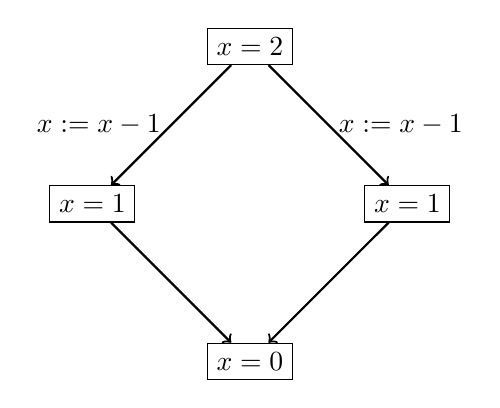
\begin{tikzpicture}
    \node[draw] (start)  at (2, 4) {$x=2$};
    \node[draw] (left)   at (0, 2) {$x=1$};
    \node[draw] (right)  at (4, 2) {$x=1$};
    \node[draw] (merged) at (2, 0) {$x=0$};

    \draw[thick, ->] (start) to node[left]  {$x := x - 1$} (left);
    \draw[thick, ->] (start) to node[right] {$x := x - 1$} (right);
    \draw[thick, ->] (left)  to (merged);
    \draw[thick, ->] (right) to (merged);
  \end{tikzpicture}
  \caption{
    A counterexample showing transaction $x := x - 1$ is not invariant
    confluent with respect to the invariant $x > 0$. The top, left, and right
    states satisfy the invariant, but the bottom state does not.
  }
  \label{fig:decrement}
\end{figure}

\subsection{Formalizing the Question}\label{sec:counter-question}
Our invariant language is defined by the grammar in \figref{invariant-grammar}
which includes linear equations and inequalities over variables in a finite set
$\var$ and integer constants in $\ints$.

\begin{figure}[h]
  \centering

  \newcommand{\atom}{\textsf{atom}}
  \newcommand{\aexp}{\textsf{aexp}}
  \newcommand{\bexp}{\textsf{bexpr}}
  \begin{gather*}
    \begin{array}{rrll}
      \atom & ::= & k & \text{\emph{constants}} \\
            & |   & x & \text{\emph{variables}} \\
      &&& \\
      \aexp  & ::= & \atom         & \text{\emph{atom}} \\
             & |   & -\atom        & \text{\emph{negation}} \\
             & |   & \aexp + \aexp & \text{\emph{addition}} \\
             & |   & \aexp - \aexp & \text{\emph{subtraction}} \\
      &&& \\
      \bexp  & ::= & \aexp \leq \aexp  & \text{\emph{inequality}} \\
             & |   & \lnot \bexp       & \text{\emph{negation}} \\
             & |   & \bexp \land \bexp & \text{\emph{conjunction}} \\
             & |   & \bexp \lor \bexp  & \text{\emph{disjunction}} \\
    \end{array}
  \end{gather*}

  \caption{
    A grammar for our linear equation and linear inequality invariant language.
    Note that the comparison operators $=$, $\neq$, $<$, $>$, and $\geq$ are
    not included because they can be defined in terms of the existing
    operators.
  }
  \label{fig:invariant-grammar}
\end{figure}

A \emph{database state} is a total function $D: \var \to \ints$.  We say a
database state $D$ \emph{satisfies invariant} $I$, denoted $I(D)$, if $I$
evaluates to true after all variables in $I$ have been replaced by their
mapping in $D$. Let $\dbs$ denote the set of all database states.

A \emph{transaction} is a partial function $t: \var \rightharpoonup \ints$.
\emph{Applying a transaction} $t$ to database state $D$, denoted by $D \circ
t$, produces a new database state defined as follows:
\[
  (D \circ t)(x) \defeq \begin{cases*}
    D(x) + t(x) & $x \in \dom{}(t)$ \\
    D(x)        & otherwise
  \end{cases*}
\]
Note that transaction application is commutative. That is for all database
states $D$ and transactions $t_1$ and $t_2$, $D \circ t_1 \circ t_2 = D \circ
t_2 \circ t_1$.

A transaction chain $C$ created from a set of transactions $T$ is a sequence of
transactions $t_1, \ldots, t_n$ where $t_i \in T$ for $1 \leq i \leq n$. Let $D
\circ C$ be syntactic sugar for $D \circ t_1 \circ \cdots \circ t_n$. We say
$C$ \emph{satisfies invariant} $I$ starting at $D$, denoted $I(C @ D)$, if for
every prefix $C'$ of $C$, $D \circ C'$ satisfies invariant $I$.

A set of transactions $T$ is \iconfluent{} with respect to invariant $I$ if for
all database states $D$ and chains $C_1$ and $C_2$ created from $T$, if $D$
satisfies $I$, $C_1$ satisfies $I$ starting at $D$, and $C_2$ satisfies $I$
starting at $D$, then $D \circ C_1 \circ C_2$ satisfies $I$.

\subsection{A Geometric Interpretation}\label{sec:counter-geometry}
\newcommand{\inva}{x + y \geq 0}
\newcommand{\invb}{x - y \leq 0}
\newcommand{\invc}{y \geq 1}
\newcommand{\invd}{y \geq 3}
\newcommand{\inv}{(\inva \land \invb \land \invc) \lor (\invd)}

Sometimes, we can eyeball whether a transaction is \iconfluent{} with respect
to an invariant. Other times, not so much. For example, which transactions are
\iconfluent{} with respect to the invariant $\inv$? It's not immediately
clear.  Surprisingly, we can interpret the question ``Is $T$ \iconfluent{} with
respect to $I$?'' geometrically, and doing so will make answering the question
much easier!

Consider an invariant $I$ over $n$ variables $x_1, \ldots, x_n$. If we imagine
the values of the $n$ variables as an $n$-dimensional point, then we can draw
the set of points in $\ints^n$ that satisfy $I$. In fact, if we canonicalize
$I$ by eliminating negations and converting to conjunctive normal form, then
the set of points satisfying $I$ is the intersection (for $\land)$ and union
(for $\lor$) of the solutions to a set of linear equations and inequalities,
which is always straightforward to draw. For example, the set of points
satisfying $\inv$ is shown in \figref{geometric-example}.

\begin{figure}
  \newenvironment{griddedpic}{
    \begin{tikzpicture}[scale=0.4]
      \clip (-4, -1) rectangle (4, 4);
  }{
      \draw (-4, -1) grid (4, 4);
      \draw[ultra thick] (-4, 0) -- (4, 0);
      \draw[ultra thick] (0, -1) -- (0, 4);
    \end{tikzpicture}
  }

  \begin{subfigure}[b]{0.24\textwidth}
    \centering
    \begin{griddedpic}
      \fill[red, opacity=0.4]
        (-10, 10) -- (10, -10) -- (10, 10) -- cycle;
    \end{griddedpic}
    \caption{$\inva$}
  \end{subfigure}
  \begin{subfigure}[b]{0.24\textwidth}
    \centering
    \begin{griddedpic}
      \fill[blue, opacity=0.4]
        (-10, -10) -- (10, 10) -- (-10, 10) -- cycle;
    \end{griddedpic}
    \caption{$\invb$}
  \end{subfigure}
  \begin{subfigure}[b]{0.24\textwidth}
    \centering
    \begin{griddedpic}
      \fill[green, opacity=0.4]
        (-10, 1) -- (10, 1) -- (10, 10) -- (-10, 10) -- cycle;
    \end{griddedpic}
    \caption{$\invc$}
  \end{subfigure}
  \begin{subfigure}[b]{0.24\textwidth}
    \centering
    \begin{griddedpic}
      \fill[orange, opacity=0.4]
        (-10, 3) -- (10, 3) -- (10, 10) -- (-10, 10) -- cycle;
    \end{griddedpic}
  \caption{$\invd$}

  \end{subfigure}
  \begin{subfigure}[b]{\textwidth}
    \centering
    \begin{griddedpic}
      \fill[purple, opacity=0.4]
        (-1, 1) -- (-3, 3) -- (-10, 3) -- (-10, 10) -- (10, 10) -- (10, 3) --
        (3, 3) -- (1, 1) -- cycle;
    \end{griddedpic}
    \caption{$\inv$}
  \end{subfigure}

  \caption{An illustration of the solution to $\inv$.}
  \label{fig:geometric-example}
\end{figure}

Next, we can imagine a transaction $t$ as an $n$-dimensional vector $(k_{x_1},
\ldots, k_{x_n})$ where $t$ adds constant $k_{x_i}$ to variable $x_i$. Now, the
question of whether a set of transactions $T$ is \iconfluent{} with respect to
invariant $I$ has been reduced to the following question. Starting at an
arbitrary point $D$ in the solution space of $I$, if we can add vectors $t^1_1,
t^1_2, \ldots, t^1_m$ to $D$ and vectors $t^2_1, t^2_2, \ldots, t^2_n$ to $D$
all while staying in the solution space of $I$, then are we guaranteed that $D
+ t^1_1 + t^1_2 + \ldots + t^1_m + t^2_1 + t^2_2 + \ldots + t^2_n$ is in the
solution space of $I$?

Turning again to our example in \figref{geometric-example}, it is now clear
that any transaction $(k_x, k_y)$ where $y \geq 0$ and $|x| \leq y$ is
\iconfluent{} with respect to $\inv$. These are the vectors that point up and
not too far left or right.

\subsection{One is Enough}\label{sec:counter-one}
Define a set of transactions $T$ to be $k$-\iconfluent{} with respect to
invariant $I$ if for all database states $D$ and chains $C_1$ and $C_2$ created
from $T$ of length at most $k$, if $D$ satisfies $I$, $C_1$ satisfies $I$
starting at $D$, and $C_2$ satisfies $I$ starting at $D$, then $D \circ
C_1 \circ C_2$ satisfies $I$.
%
A set of transactions $T$ is \iconfluent{} with respect to an invariant $I$ if
it is $k$-\iconfluent{} for all $k$. Thus, when reasoning about \iconfluent{}
transactions, we have to consider potentially large transaction chains which
can be a bit brain boggling. Reasoning about 1-\iconfluence{} is much easier
because we only have to consider a pair of transactions at a time. This
subsection proves a convenient lemma that 1-\iconfluence{} and \iconfluence{}
are equivalent.

\begin{theorem}\label{thm:one-is-enough}
  For all sets of transactions $T$ and invariants $I$, T is 1-\iconfluent{} if
  and only if it is \iconfluent{}.
\end{theorem}
\begin{proof}
  The reverse direction is immediate from the definition of \iconfluence{}. For
  the forward direction, consider a set of transactions $T$ that is
  1-\iconfluent{} with respect to an invariant $I$. Consider an arbitrary
  database state $D$ and two chains $C^t = t_1, t_2, \ldots, t_m$ and $C^u =
  u_1, u_2, \ldots, u_n$ such that $D$ satisfies $I$, $C^t$ satisfies $I$
  starting at $D$, and $C^u$ satisfies $I$ starting at $D$. We show $D \circ
  C^t \circ C^u$ satisfies $I$.

  Let $C^z_j$ denote the prefix of $C^z$ of length $j$. We show by strong
  mathematical induction on $i$, that $D \circ C^t_j \circ C^u_k$ satisfies $I$
  for all $0 \leq j \leq m$, $0 \leq k \leq n$, and $0 \leq i = j + k \leq n +
  m$.
  %
  The base case, when $i = 0$, is trivial. $j = k = 0$, and $D \circ C^t_0
  \circ C^u_0 = D$ which satisfies $I$ by assumption.
  %
  For the inductive step, we wish to show for arbitrary $0 \leq j \leq m$, $0
  \leq k \leq n$, and $i = j + k$ that $D \circ C^t_j \circ C^u_k$ satisfies
  $I$. If $j = 0$, then $D \circ C^t_0 \circ C^u_k = D \circ C^u_k$ satisfies
  $I$ by the assumption that $C^u$ satisfies $I$ starting at $D$, and likewise
  for when $k = 0$. Now consider $j, k > 0$. By the inductive hypothesis, we
  know
    (1) $D \circ C^t_{j-1} \circ C^u_{k-1}$,
    (2) $D \circ C^t_{j-1} \circ C^u_{k}$, and
    (3) $D \circ C^t_{j}   \circ C^u_{k-1}$
  all satisfy $I$. If we let (1) be our initial database state, $t_j$ be one
  chain, and $u_k$ be the other chain, then the 1-\iconfluence{} of $T$ tells
  us that $(1) \circ t_j \circ u_k = D \circ C^t_j \circ C^u_k$ satisfies
  $I$.
\end{proof}

\newcommand{\baseedges}{
  \begin{scope}[on background layer]
    \draw[txn] (03) -- (13) node[midway, above]{$u_1$};
    \draw[txn] (13) -- (23) node[midway, above]{$u_2$};
    \draw[txn] (23) -- (33) node[midway, above]{$u_3$};
    \draw[txn] (03) -- (02) node[midway, left]{$t_1$};
    \draw[txn] (02) -- (01) node[midway, left]{$t_2$};
    \draw[txn] (01) -- (00) node[midway, left]{$t_3$};
    \draw[dtxn] (00) -- (30);
    \draw[dtxn] (33) -- (30);
  \end{scope}
}

\begin{figure}[h]
  \centering
  \newcommand{\onescale}{1.1}

  \begin{subfigure}[b]{0.49\textwidth}
    \centering
    \begin{tikzpicture}[scale=\onescale]
      \foreach \x/\y in {
             1/3, 2/3, 3/3,
        0/2,
        0/1,
        0/0%
      } {
        \inode{\x\y}{\x, \y}
      }
      \foreach \x/\y in {0/3} {
        \inode[red]{\x\y}{\x, \y}
      }
      \nnode{30}{3, 0}
      \baseedges{}
    \end{tikzpicture}
    \caption{$i = 0$}
    \label{fig:one-is-enough-base}
  \end{subfigure}
  \begin{subfigure}[b]{0.49\textwidth}
    \centering
    \begin{tikzpicture}[scale=\onescale]
      \foreach \x/\y in {
        0/3,      2/3, 3/3,
        %
        0/1,
        0/0%
      } {
        \inode{\x\y}{\x, \y}
      }
      \foreach \x/\y in {0/2, 1/3} {
        \inode[red]{\x\y}{\x, \y}
      }
      \nnode{30}{3, 0}
      \baseedges{}
    \end{tikzpicture}
    \caption{$i=1$}
    \label{}
  \end{subfigure}

  \begin{subfigure}[b]{0.3\textwidth}
    \centering
    \begin{tikzpicture}[scale=\onescale]
      \foreach \x/\y in {
        0/3, 1/3,      3/3,
        0/2,
        %
        0/0%
      } {
        \inode{\x\y}{\x, \y}
      }
      \foreach \x/\y in {0/1, 1/2, 2/3} {
        \inode[red]{\x\y}{\x, \y}
      }
      \nnode{30}{3, 0}
      \baseedges{}
      \draw[txn] (02) -- (12) node[midway, above] {$u_1$};
      \draw[txn] (13) -- (12) node[midway, left]  {$t_1$};
    \end{tikzpicture}
    \caption{$i=2$}
    \label{}
  \end{subfigure}
  \begin{subfigure}[b]{0.3\textwidth}
    \centering
    \begin{tikzpicture}[scale=\onescale]
      \foreach \x/\y in {
        0/3, 1/3, 2/3,
        0/2, 1/2,
        0/1%
        %
      } {
        \inode{\x\y}{\x, \y}
      }
      \foreach \x/\y in {0/0, 1/1, 2/2, 3/3} {
        \inode[red]{\x\y}{\x, \y}
      }
      \nnode{30}{3, 0}
      \baseedges{}
      \draw[txn] (02) -- (12) node[midway, above] {$u_1$};
      \draw[txn] (13) -- (12) node[midway, left]  {$t_1$};
      \draw[txn] (01) -- (11) node[midway, above] {$u_1$};
      \draw[txn] (12) -- (11) node[midway, left]  {$t_2$};
      \draw[txn] (12) -- (22) node[midway, above] {$u_2$};
      \draw[txn] (23) -- (22) node[midway, left]  {$t_1$};
    \end{tikzpicture}
    \caption{$i=3$}
    \label{}
  \end{subfigure}
  \begin{subfigure}[b]{0.3\textwidth}
    \centering
    \begin{tikzpicture}[scale=\onescale]
      \foreach \x/\y in {
        0/3, 1/3, 2/3, 3/3,
        0/2, 1/2, 2/2,
        0/1, 1/1,
        0/0%
      } {
        \inode{\x\y}{\x, \y}
      }
      \foreach \x/\y in {1/0, 2/1, 3/2} {
        \inode[red]{\x\y}{\x, \y}
      }
      \nnode{30}{3, 0}
      \baseedges{}
      \draw[txn] (02) -- (12) node[midway, above] {$u_1$};
      \draw[txn] (13) -- (12) node[midway, left]  {$t_1$};
      \draw[txn] (01) -- (11) node[midway, above] {$u_1$};
      \draw[txn] (12) -- (11) node[midway, left]  {$t_2$};
      \draw[txn] (12) -- (22) node[midway, above] {$u_2$};
      \draw[txn] (23) -- (22) node[midway, left]  {$t_1$};
      \draw[txn] (00) -- (10) node[midway, above] {$u_1$};
      \draw[txn] (11) -- (10) node[midway, left]  {$t_3$};
      \draw[txn] (11) -- (21) node[midway, above] {$u_2$};
      \draw[txn] (22) -- (21) node[midway, left]  {$t_2$};
      \draw[txn] (22) -- (32) node[midway, above] {$u_3$};
      \draw[txn] (33) -- (32) node[midway, left]  {$t_1$};
    \end{tikzpicture}
    \caption{$i=4$}
    \label{}
  \end{subfigure}

  \begin{subfigure}[b]{0.49\textwidth}
    \centering
    \begin{tikzpicture}[scale=\onescale]
      \foreach \x/\y in {
        0/3, 1/3, 2/3, 3/3,
        0/2, 1/2, 2/2, 3/2,
        0/1, 1/1, 2/1,
        0/0, 1/0%
      } {
        \inode{\x\y}{\x, \y}
      }
      \foreach \x/\y in {2/0, 3/1} {
        \inode[red]{\x\y}{\x, \y}
      }
      \nnode{30}{3, 0}
      \baseedges{}
      \draw[txn] (02) -- (12) node[midway, above] {$u_1$};
      \draw[txn] (13) -- (12) node[midway, left]  {$t_1$};
      \draw[txn] (01) -- (11) node[midway, above] {$u_1$};
      \draw[txn] (12) -- (11) node[midway, left]  {$t_2$};
      \draw[txn] (12) -- (22) node[midway, above] {$u_2$};
      \draw[txn] (23) -- (22) node[midway, left]  {$t_1$};
      \draw[txn] (00) -- (10) node[midway, above] {$u_1$};
      \draw[txn] (11) -- (10) node[midway, left]  {$t_3$};
      \draw[txn] (11) -- (21) node[midway, above] {$u_2$};
      \draw[txn] (22) -- (21) node[midway, left]  {$t_2$};
      \draw[txn] (22) -- (32) node[midway, above] {$u_3$};
      \draw[txn] (33) -- (32) node[midway, left]  {$t_1$};
      \draw[txn] (10) -- (20) node[midway, above] {$u_2$};
      \draw[txn] (21) -- (20) node[midway, left]  {$t_3$};
      \draw[txn] (21) -- (31) node[midway, above] {$u_3$};
      \draw[txn] (32) -- (31) node[midway, left]  {$t_2$};
    \end{tikzpicture}
    \caption{$i=5$}
    \label{}
  \end{subfigure}
  \begin{subfigure}[b]{0.49\textwidth}
    \centering
    \begin{tikzpicture}[scale=\onescale]
      \foreach \x/\y in {
        0/3, 1/3, 2/3, 3/3,
        0/2, 1/2, 2/2, 3/2,
        0/1, 1/1, 2/1, 3/1,
        0/0, 1/0, 2/0%
      } {
        \inode{\x\y}{\x, \y}
      }
      \inode[red]{30}{3, 0}
      \baseedges{}
      \draw[txn] (02) -- (12) node[midway, above] {$u_1$};
      \draw[txn] (13) -- (12) node[midway, left]  {$t_1$};
      \draw[txn] (01) -- (11) node[midway, above] {$u_1$};
      \draw[txn] (12) -- (11) node[midway, left]  {$t_2$};
      \draw[txn] (12) -- (22) node[midway, above] {$u_2$};
      \draw[txn] (23) -- (22) node[midway, left]  {$t_1$};
      \draw[txn] (00) -- (10) node[midway, above] {$u_1$};
      \draw[txn] (11) -- (10) node[midway, left]  {$t_3$};
      \draw[txn] (11) -- (21) node[midway, above] {$u_2$};
      \draw[txn] (22) -- (21) node[midway, left]  {$t_2$};
      \draw[txn] (22) -- (32) node[midway, above] {$u_3$};
      \draw[txn] (33) -- (32) node[midway, left]  {$t_1$};
      \draw[txn] (10) -- (20) node[midway, above] {$u_2$};
      \draw[txn] (21) -- (20) node[midway, left]  {$t_3$};
      \draw[txn] (21) -- (31) node[midway, above] {$u_3$};
      \draw[txn] (32) -- (31) node[midway, left]  {$t_2$};
      \draw[txn] (20) -- (30) node[midway, above] {$u_3$};
      \draw[txn] (31) -- (30) node[midway, left]  {$t_3$};
    \end{tikzpicture}
    \caption{$i=6$}
    \label{}
  \end{subfigure}

  \caption{Illustration of the proof of \thmref{one-is-enough}.}
  \label{fig:one-is-enough}
\end{figure}

\figref{one-is-enough} visualizes the proof of \thmref{one-is-enough} using
\emph{state diagrams}. In a state diagram, each dot represents a database state
$D$, and we draw an edge labelled $t$ from database $D$ to database $D'$ if $D
\circ t = D'$. We circle a database dot if we know it satisfies the invariant
and leave it uncircled otherwise.

\figref{one-is-enough} illustrates an initial database $D$ (top-left dot), a
chain $C^t = \set{t_1, t_2, t_3}$ (the left edge), a chain $C^u = \set{u_1,
u_2, u_3}$ (the top edge), and $D \circ C^t \circ C^u$ (the bottom-right dot).
By assumption, we know $D$, $D \circ C^t_1$, $D \circ C^t_2$, $D \circ C^t$, $D
\circ C^u_1$, $D \circ C^u_2$, and $D \circ C^u$ satisfy the invariant, and we
want to show that $D \circ C^t \circ C^u$ satisfies the invariant.
\figref{one-is-enough-base} illustrates the base case of
\thmref{one-is-enough}; each of the other six state diagrams illustrate one
inductive step of \figref{one-is-enough}. In each inductive step, we exploit
the fact that $T$ is 1-\iconfluent{} to conclude that some set of intermediate
databases satisfy the invariant.

\subsection{A Solution}\label{sec:solution}
This section posed the question: how do we write an algorithm to decide whether
a set of PN-Counter increment/decrement transactions are \iconfluent{} with
respect to an invariant expressed as a formula of linear equations and
inequalities?  Now that we're armed with an intuitive
(\secref{counter-overview}) and formal (\secref{counter-question})
understanding of the problem, a geometric interpretation
(\secref{counter-geometry}), and a useful lemma (\secref{counter-one}), we're
in a perfect position to present a solution!

In a nutshell, our algorithm translates a set of transactions $T$ and invariant
$I$ into a universally quantified invariant $F$ in prenex normal form where $F$
is a tautology if and only if $T$ is 1-\iconfluent{} with respect to $I$. Thus,
by \thmref{one-is-enough}, $F$ is a tautology if and only if $T$ is
\iconfluent{} with respect to $I$. Our algorithm then uses Z3 \cite{de2008z3}
to check if $F$ is a tautology.

The algorithm for constructing $F$ is best explained by way of example.
Consider a simple case where $I = x + y \geq 0$, and $T$ consists of a single
transaction $t$ which increments $x$ by 1 and $y$ by 2. Our algorithm
constructs the following formula
\begin{align}
  & \forall x.\> \forall y.\>                \label{eq:vars} \\
  & \forall dx_1.\> \forall dy_1.\>          \label{eq:dvars1} \\
  & \forall dx_2.\> \forall dy_2.\>          \label{eq:dvars2} \\
  & (dx_1 = 1 \land dy_1 = 2) \land {}       \label{eq:t1} \\
  & (dx_2 = 1 \land dy_2 = 2) \implies {}    \label{eq:t2} \\
  & x + y \geq 0 \implies {}                 \label{eq:i} \\
  & x + dx_1 + y + dy_1 \geq 0 \implies {}   \label{eq:i1} \\
  & x + dx_2 + y + dy_2 \geq 0 \implies {}   \label{eq:i2} \\
  & x + dx_1 + dx_2 + y + dy_1 + dy_2 \geq 0 \label{eq:i12}
\end{align}
where
\begin{itemize}
  \item
    \eqref{eq:vars} universally quantifies the free variables in $I$.

  \item
    \eqref{eq:dvars1} and \eqref{eq:dvars2} universally quantify variables
    $dx_1$ and $dx_2$ for each free variable $x$ in the invariant $I$.
    Intuitively, if the invariant has free variables $a, \ldots, z$, then the
    variables $da_1, \ldots, dz_1$ represent the increments and decrements of
    one transaction and $da_2, \ldots, dz_2$ represent the increments and
    decrements of another transaction.

  \item
    \eqref{eq:t1} and \eqref{eq:t2} assert that $dx_1$, $dy_1$, $dx_2$, and
    $dy_2$ must take on values consistent with $t$. Specifically, $x$ must be
    incremented by 1, and $y$ must be incremented by $2$.

  \item
    \eqref{eq:i} is $I$. Intuitively, it predicates our implication on the
    assumption that the current database state satisfies the invariant.

  \item
    \eqref{eq:i1} is $I$ with every variable $x$ replaced with $x + dx_1$.
    Intuitively, it predicates our implication on the assumption that if we
    apply the first transaction, our database still satisfies the invariant.
    \eqref{eq:i2} is symmetric to \eqref{eq:i1} but for the second transaction
    instead of the first.

  \item
    \eqref{eq:i12} is $I$ with every variable $x$ replaced with $x + dx_1 +
    dx_2$. Intuitively, it says that if we apply both the transactions, we
    continue to satisfy our invariant.
\end{itemize}

To summarize, the formula encodes the statement that for all database state
$(x, y)$ for all transactions $t_1 = (dx_1, dy_1) \in T$, and for all
transactions $t_2 = (dx_2, dy_2) \in T$, if $(x, y)$, $(x + dx_1, y + dy_1)$,
and $(x + dx_2, y + dy_2)$ satisfy the invariant, then so does $(x + dx_1 +
dx_2, y + dy_1 + dy_2)$. In other words, the formula is nothing more than a
restatement of the definition of 1-\iconfluence!

\subsection{\imp{} Transactions}\label{sec:imptxns}
So far, we've modelled a transaction $t: \var \rightharpoonup \ints$ as a
partial function from variables to integers. Intuitively, a transaction chooses
some \emph{fixed} subset of variables and increments and decrements each by
some \emph{fixed} amount. We'll call these kinds of transactions \emph{fixed
transactions}. While simple, fixed transactions are \emph{inexpressive}. We can
model, for example, a transaction that increments $x$ by 42 and decrements $y$
by 14, but we \emph{can't} model a transaction that increments $y$ by $x$ or a
transaction that increments $y$ by 1 whenever $x$ is positive and increments
$z$ whenever $x$ is negative.

In this subsection, we introduce a simple imperative programming language
\imp{}\footnote{That's IMP \cite{winskel1993formal} with an $\iinvariant{}$.}.
Instead of looking at fixed transactions, we'll look at \imp{}
transactions---transactions written in \imp{}---and ask ourselves the question
of how do determine whether a set of \imp{} transactions is \iconfluent{} with
respect to some invariant.

\begin{figure}[h]
  \centering
  \begin{gather*}
    \begin{array}{rrll}
      \impaexp\;
        a & ::= & k       & \text{\emph{constant}} \\
          & |   & x       & \text{\emph{variable}} \\
          & |   & read(x) & \text{\emph{database read}} \\
          & |   & a + a   & \text{\emph{addition}} \\
          & |   & a - a   & \text{\emph{subtraction}} \\
          & |   & - a     & \text{\emph{negation}} \\
      &&& \\
      \impbexp\;
        b & ::= & \textsf{true}  & \text{\emph{true}} \\
          & |   & \textsf{false} & \text{\emph{false}} \\
          & |   & a \odot a      & \text{\emph{linear constraint}} \\
          & |   & \lnot b        & \text{\emph{negation}} \\
          & |   & b \lor b       & \text{\emph{disjunction}} \\
          & |   & b \land b      & \text{\emph{conjunction}} \\
      &&& \\
      \impcom\;
        c  & ::= & \impskip        & \text{\emph{skip}} \\
           & |   & x := a          & \text{\emph{assignment}} \\
           & |   & add(x, a)       & \text{\emph{database adds}} \\
           & |   & c; c            & \text{\emph{sequence}} \\
           & |   & \impif{b}{c}{c} & \text{\emph{conditional}} \\
      &&& \\
      \odot & ::= & =    \vert
                    \neq \vert
                    <    \vert
                    \leq \vert
                    >    \vert
                    \geq & \text{\emph{comparator}}
    \end{array}
  \end{gather*}

  \caption{
    A grammar for \imp{}: a simple imperative transaction language inspired by
    IMP \cite{winskel1993formal} and $\mathcal{L}$ \cite{roy2015homeostasis}.
    The language consists of arithmetic expressions $\impaexp{}$, boolean
    expressions $\impbexp{}$, and commands $\impcom{}$.
  }
  \label{fig:imp-grammar}
\end{figure}

The syntax of \imp{} is defined by the grammar in \figref{imp-grammar}. The
semantics of \imp{} can be defined denotationally. That is, we can define a
denotational semantics $\denote{\cdot}$ where for an \imp{} program $c$,
$\denote{c}: (\var \to \ints) \to (\var \rightharpoonup \ints)$ is a function
from a database to a fixed transaction. Defining these semantics is left as an
exercise to the reader.  See \cite{cs6110sp2016lecture19} for guidance.
\todo{Define, explicitly, the denotational semantics if need be.}

\emph{Applying an \imp{} transaction} $c$ to database state $D$, denoted by $D
\circ c$, is defined as $D \circ c \defeq D \circ (\denote{c}(D))$.  Note that
unlike fixed transaction application, \imp{} transaction application is
\emph{not} commutative! For example, consider the database $D=\set{(x, 0)}$ and
\imp{} transactions $c_1 = add(x, 1)$ and $c_2 = add(x, read(x))$.
\[
  D \circ c_1 \circ c_2
    = \set{(x, 1)} \circ c_2
    = \set{(x, 2)}
    \neq \set{(x, 1)}
    = \set{(x, 0)} \circ c_1
    = D \circ c_2 \circ c_1
\]

An \imp{} transaction chain $B$ created from a set of \imp{} transactions $T$
is a sequence of \imp{} transactions $c_1, \ldots, c_n$ where $c_i \in T$ for
$1 \leq i \leq n$. Each \imp{} transaction chain $B$ starting with database
state $D$ has a corresponding fixed transaction chain $C$ denoted
$\denote{B}(D)$. Let $D_i = D \circ c_1 \circ \cdots \circ c_i$. Then, the
corresponding fixed transaction chain is $\denote{c_1}(D_0), \ldots,
\denote{c_n}(D_{n-1})$. We say $B$ \emph{satisfies invariant} $I$ starting at
$D$, denoted $I(B@D)$, if the corresponding fixed transaction chain $C$
satisfies invariant $I$ starting at $D$.

We say a set of \imp{} transactions $T$ is \iconfluent{} with respect to
invariant $I$ if for all database states $D$, all \imp{} chains $B_1$ and $B_2$
created from $T$, and corresponding fixed transaction chains $C_1$ and $C_2$,
if $D$ satisfies $I$, $B_1$ satisfies $I$ starting at $D$, and $B_2$ satisfies
$I$ starting at $D$, then $D \circ C_1 \circ C_2$ satisfies $I$. We define
$k$-\iconfluence{} similar to how we did in \secref{counter-one}.

Now that we've formalized what it means for a set of \imp{} transactions to be
\iconfluent{} with respect to some invariant, how do we determine
\iconfluence{} algorithmically? One initial hunch would be to apply the same
technique from \secref{solution} with slight modification. Unfortunately,
\clmref{imp-1-iconfluence} presents a challenge.

\begin{claim}\label{clm:imp-1-iconfluence}
  For \imp{} transactions, $1$-\iconfluence $\centernot \implies$ \iconfluence.
\end{claim}
\begin{proof}
  Consider the following invariant and \imp{} transactions:
  \begin{align*}
    I &\defeq
      (-2 \leq x \leq 2 \land y = 0) \lor (x = 1 \land 0 \leq y \leq 2) \\
    c_1 &\defeq \impif{x = 0 \land y = 0}{
      add(x, 1)
    }{\impif{x = 1 \land y = 0} {
      add(y, 1)
    }{
      \impskip
    }} \\
    c_2 &\defeq \impif{x = 0 \land y = 0}{
      add(x, -1)
    }{\impif{x = 1 \land y = 0} {
      add(y, 1)
    }{
      \impskip
    }}
  \end{align*}

  $T = \set{c_1, c_2}$ is $1$-\iconfluent{} with respect to $I$, but not
  $2$-\iconfluent{} with respect to $I$. Proving this is easiest if we
  interpret \imp{} transactions geometrically, as we did with fixed
  transactions.

  As before, invariants over $n$ variables correspond to a set of points in
  $\ints^n$; for example, $I$ is visualized in \figref{iviz}. An \imp{}
  transaction $c$ can be thought of as vector valued functions $c: \ints^n \to
  \ints^n$ that maps each point in $\ints^n$ to a $n$-dimensional vector. For
  example, $c_1$ and $c_2$ are visualized in \figref{c1viz} and \figref{c2viz}.
  The visualization of $c_1$ has two vectors. The $(1, 0)$ vector originating
  at the origin corresponds to $c_1$ adding $1$ to $x$ whenever $x = 0 \land y
  = 0$. Similarly, the $(0, 1)$ originating at $(1, 0)$ corresponds to $c_1$
  adding $1$ to $y$ whenever $x = 1 \land y = 0$.

  Using this geometric interpretation, it's easy to perform a brute-force check
  that $T$ is $1$-\iconfluent with respect to $I$. However, consider the
  transaction chains $B_1 = \set{c_1, c_2}$ and $B_2 = \set{c_2, c_1}$ starting
  in database state $D = (0, 0)$. We know that
  \begin{itemize}
    \item $D = (0, 0)$ satisfies $I$,
    \item $D \circ c_1 = (0, 1)$ satisfies $I$,
    \item $D \circ c_1 \circ c_2 = (1, 1)$ satisfies $I$,
    \item $D \circ c_2 = (-1, 0)$ satisfies $I$, and
    \item $D \circ c_2 \circ c_1 = (-1, 0)$ satisfies $I$,
  \end{itemize}
  but $D \circ C_1 \circ C_2 = D \circ (1, 0) \circ (0, 1) \circ (-1, 0) \circ
  (0, 0) = (0, 1)$ does not satisfy $I$. Therefore, $T$ is not 2-\iconfluent
  with respect to $I$ and is therefore not \iconfluent with respect to $I$.
\end{proof}

\todo{
  \clmref{imp-1-iconfluence} puts us in a bit of pickle. Think about how to get
  out of it. Maybe we check for $k$-\iconfluence for some $k$ and then use a
  reservation system to bound the amount of divergence between replicas? That
  doesn't seem to make sense for a system with high transaction throughput.
  Maybe there are some other tricks we can play?
}

\tikzstyle{point}=[shape=circle, fill=blue, opacity=0.75]
\tikzstyle{vec}=[->, ultra thick, red, shorten >=0.1cm]
\begin{figure}[h]
  \centering

  \newcommand{\gridandpoints}{
    \draw[ultra thick] (-2, 0) -- (2, 0);
    \draw[ultra thick] (0, 0) -- (0, 2);
    \draw (-2, 0) grid (2, 2);
    \foreach \x/\y in {-2/0, -1/0, 0/0, 1/0, 2/0, 1/1, 1/2} {
      \node[point] (\x-\y) at (\x, \y) {};
    }
  }

  \begin{subfigure}[c]{0.3\textwidth}
    \centering
    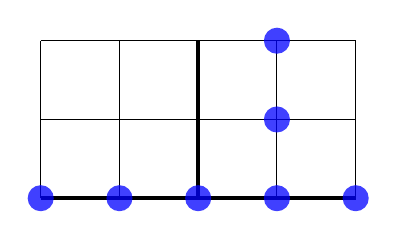
\begin{tikzpicture}
      \gridandpoints{}
    \end{tikzpicture}
    \caption{Visualization of $I$.}
    \label{fig:iviz}
  \end{subfigure}
  \begin{subfigure}[c]{0.3\textwidth}
    \centering
    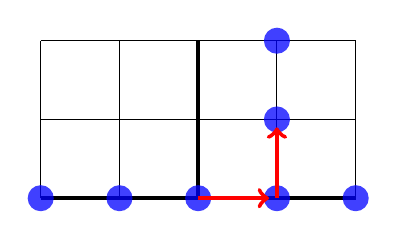
\begin{tikzpicture}
      \gridandpoints{}
      \draw[vec] (0, 0) -- (1, 0);
      \draw[vec] (1, 0) -- (1, 1);
    \end{tikzpicture}
    \caption{Visualization of $c_1$.}
    \label{fig:c1viz}
  \end{subfigure}
  \begin{subfigure}[c]{0.3\textwidth}
    \centering
    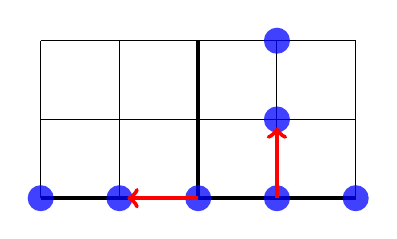
\begin{tikzpicture}
      \gridandpoints{}
      \draw[vec] (0, 0) -- (-1, 0);
      \draw[vec] (1, 0) -- (1, 1);
    \end{tikzpicture}
    \caption{Visualization of $c_2$.}
    \label{fig:c2viz}
  \end{subfigure}

  \caption{
    A geometric interpretation of $I$, $c_1$, and $c_2$ from
    \clmref{imp-1-iconfluence}. $I$ corresponds to a subset of $\ints^2$. $c_1$
    and $c_2$ correspond to vector valued functions of type $\ints^2 \to
    \ints^2$.
  }
  \label{fig:icviz}
\end{figure}

\subsection{\wimp{} Transactions}\label{sec:datatxns}
We began this section by looking at fixed transactions and concluded in
\thmref{one-is-enough} that if a set of fixed transactions is 1-\iconfluent{}
with respect to an invariant $I$, then it is also \iconfluent{}. Then in
\secref{imptxns}, we enriched transactions from simple fixed partial functions
to full-blown programs written in \imp{}. Unfortunately, this increase in
expressiveness came at the cost of the nice fact that 1-\iconfluence{} is
equivalent to \iconfluence{}, as we saw in \clmref{imp-1-iconfluence}.

Perhaps \imp{} is too powerful of a transaction language. In particular, it has
two powerful features that fixed transactions do not have. First, \imp{} has
conditionals allowing the control flow of an \imp{} program to depend on the
database against which it is run. Second, even without conditionals, the
behavior of an \imp{} transaction can still depend on the database state
against which it is run. For example, the behavior of the transaction $add(x,
read(x))$ depends on the initial value of $x$, even though the transaction does
not use a conditional.

Perhaps if we strip \imp{} of some its features, we'll regain the equivalence
of 1-\iconfluence{} and \iconfluence{}. That is, perhaps there is an
intermediate language more powerful than fixed transactions but weaker than
\imp{} for which 1-\iconfluence{} is equivalent to \iconfluence{}.

In this subsection, we'll consider one such language, \wimp{}: a weakened
version of \imp{}. Then, we'll conclude that for \wimp{}---as for
\imp{}---1-\iconfluence{} does not imply \iconfluence{}.

Formally, \wimp{} is \imp{} without variables, boolean expressions, skip,
assignment, and conditionals. Moreover, each database variable can be added to
at most once. Essentially, \wimp{} programs get to add a single arithmetic
expression to each database variable. While weaker than \imp{} programs,
\wimp{} programs are more powerful than fixed transactions because arithmetic
expressions can include database reads and therefore \wimp{} programs can
depend on the initial state of the database. In fact, if we remove database
reads from \wimp{}, we get a language of fixed transactions.

Since \wimp{} is a subset of \imp{}, all the definitions from \imp{} carry over
directly for \wimp{}. Also note that like \imp{}, \wimp{} transaction
application is not commutative.

As mentioned above, \wimp{} is not weak enough to enjoy the equivalence of
1-\iconfluence{} and \iconfluence{}: a fact we now prove.

\begin{claim}\label{clm:wimp-1-iconfluence}
  For \wimp{} transactions, $1$-\iconfluence $\centernot \implies$ \iconfluence.
\end{claim}
\begin{proof}
  Consider the following invariant and \wimp{} transactions:
  \begin{align*}
    I   &\defeq x \neq 0 \lor y = 0 \\
    c_1 &\defeq y.add(1) \\
    c_2 &\defeq x.add(read(x) + 1) \\
    c_3 &\defeq x.add(read(x) - 1)
  \end{align*}

  As usual, we can visualize invariants and transactions geometrically, as
  shown in \figref{wimp-icviz}. We can perform a brute-force case analysis over
  all pairs of transactions and all points to show $T = \set{c_1, c_2, c_3}$ is
  1-\iconfluent{} with respect to $I$. This is left as exercise to the reader.

  However, consider the \wimp{} chains $B_1 = \set{c_2, c_1}$ and $B_2 =
  \set{c_3, c_1}$ in database $D = (0, 0)$. We know that
  \begin{itemize}
    \item $D = (0, 0)$ satisfies $I$,
    \item $D \circ c_2 = (1, 0)$ satisfies $I$,
    \item $D \circ c_2 \circ c_1 = (1, 1)$ satisfies $I$,
    \item $D \circ c_3 = (-1, 0)$ satisfies $I$, and
    \item $D \circ c_3 \circ c_1 = (-1, 1)$ satisfies $I$,
  \end{itemize}
  but $D \circ C_1 \circ C_2 = D \circ (1, 0) \circ (0, 1) \circ (-1, 0) \circ
  (0, 1) = (0, 2)$ does not satisfy $I$. Therefore, $T$ is not 2-\iconfluent
  with respect to $I$ and is therefore not \iconfluent with respect to $I$.
\end{proof}

\todo{
  We're in a pickle again! I think this result also might suggest that the
  claims in \cite{balegas2015putting} are wrong? More likely, I'm
  misunderstanding the paper.
}

\newcommand{\width}{2}
\newcommand{\smallwidth}{1}
\newcommand{\height}{2}

\newcommand{\gridxy}{
  \draw[ultra thick] (-\width, 0) -- (\width, 0);
  \draw[ultra thick] (0, -\height) -- (0, \height);
  \draw (-\width, -\height) grid (\width, \height);
}

\newcommand{\forxy}[1]{
  \foreach \x in {-\width, ..., -1} {
    \foreach \y in {-\height, ..., \height} { #1 } }
  \foreach \x in {1, ..., \width} {
    \foreach \y in {-\height, ..., \height} { #1 } }
  \foreach \x in {0} {
    \foreach \y in {0} { #1 } }
}

\newcommand{\forxysmall}[1]{
  \foreach \x in {-\smallwidth, ..., -1} {
    \foreach \y in {-\height, ..., \height} { #1 } }
  \foreach \x in {1, ..., \smallwidth} {
    \foreach \y in {-\height, ..., \height} { #1 } }
  \foreach \x in {0} {
    \foreach \y in {0} { #1 } }
}

\begin{figure}[h]
  \centering
  \newcommand{\thescale}{0.7}

  \begin{subfigure}[b]{0.24\textwidth}
    \centering
    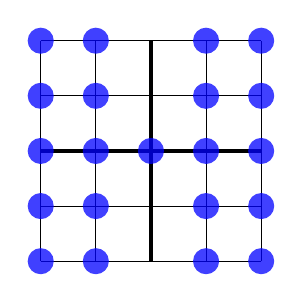
\begin{tikzpicture}[scale=\thescale]
      \gridxy{}
      \forxy{\node[point] (\x-\y) at (\x, \y) {};}
    \end{tikzpicture}
    \caption{Visualization of $I$.}
    \label{fig:wimp-iviz}
  \end{subfigure}
  \begin{subfigure}[b]{0.24\textwidth}
    \centering
    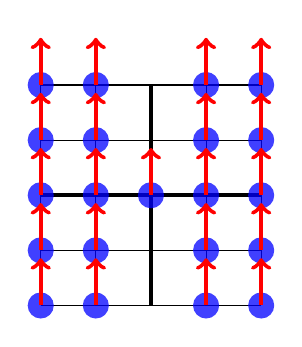
\begin{tikzpicture}[scale=\thescale]
      \gridxy{}
      \forxy{\node[point] (\x-\y) at (\x, \y) {};}
      \forxy{\draw[vec] (\x, \y) -- (\x, \y + 1);}
    \end{tikzpicture}
    \caption{Visualization of $c_1$.}
    \label{fig:wimp-c1viz}
  \end{subfigure}
  \begin{subfigure}[b]{0.24\textwidth}
    \centering
    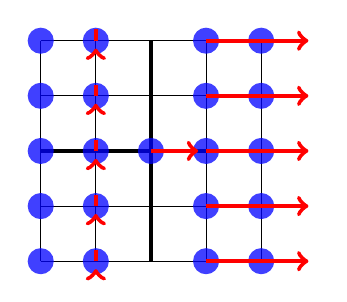
\begin{tikzpicture}[scale=\thescale]
      \gridxy{}
      \forxy{\node[point] (\x-\y) at (\x, \y) {};}
      \forxysmall{\draw[vec] (\x, \y) -- (\x + \x + 1, \y);}
    \end{tikzpicture}
    \caption{Visualization of $c_2$.}
    \label{fig:wimp-c2viz}
  \end{subfigure}
  \begin{subfigure}[b]{0.24\textwidth}
    \centering
    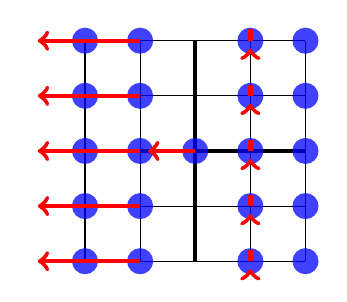
\begin{tikzpicture}[scale=\thescale]
      \gridxy{}
      \forxy{\node[point] (\x-\y) at (\x, \y) {};}
      \forxysmall{\draw[vec] (\x, \y) -- (\x + \x - 1, \y);}
    \end{tikzpicture}
    \caption{Visualization of $c_3$.}
    \label{fig:wimp-c3viz}
  \end{subfigure}

  \caption{
    A geometric interpretation of $I$, $c_1$, $c_2$, and $c_3$ from
    \clmref{wimp-1-iconfluence}. Note that the visualizations include only a
    subset of the points satisfying $I$ and that not all vectors are drawn.
  }
  \label{fig:wimp-icviz}
\end{figure}

\subsection{\iconfluence{} Alternatives}
\begin{todoitemize}
  \item \todo{\istrength $\centernot \implies$ \isafety?}
  \item \todo{\isafety $\implies$ \istrength?}
  \item \todo{\istrength $\centernot \implies$ \iconfluence?}
  \item \todo{\iconfluence $\implies$ \istrength?}
  \item \todo{\istrengthstar $\implies$ \istrength?}
  \item \todo{\istrength $\implies$ \istrengthstar?}
  \item \todo{Find something between \isafety{} and \iconfluence.}
  \item \todo{1-iconfluence with derived txns to start}
\end{todoitemize}

\begin{itemize}
  \item \textbf{0-\isafety.}
    $\forall D, D', c.\>
      I(D) \land
      I(D') \implies
      I(D \circ \denote{c}(D'))$

  \item \textbf{k-\isafety.}
    $\forall D, D', B, C, c.\>
       C = \denote{B}(D) \land
       |B| \geq k \land
       I(B @ D') \implies
       I(C @ D) \land
       I(D \circ C \circ \denote{c}{D' \circ C})$

  \item \textbf{\isafety.}
    $\forall D, D', B, C, c.\>
       C = \denote{B}(D) \land
       I(B @ D') \implies
       I(D \circ C \circ \denote{c}(D' \circ C))$

  \item \textbf{\ipreservation.} $\forall D, c.\>
       I(D) \implies
       I(D \circ \denote{c}(D))$

  \item \textbf{\iconfluence.}
    $\forall D, B_1, B_2, C_1, C_2. \>
       C_1 = \denote{B_1}(D) \land
       C_2 = \denote{B_2}(D) \land
       I(B_1 @ D) \land
       I(B_2 @ D) \implies
       I(D \circ C_1 \circ C_2)$

  \item \textbf{k-\iconfluence.}
    $\forall D, B_1, B_2, C_1, C_2. \>
       C_1 = \denote{B_1}(D) \land
       C_2 = \denote{B_2}(D) \land
       |B_1|, |B_2| \leq k \land
       I(B_1 @ D) \land
       I(B_2 @ D) \implies
       I(D \circ C_1 \circ C_2)$

  \item \textbf{1-\iconfluence.}
    $\forall D, c_1, c_2.\>
       I(D) \land
       I(D \circ \denote{c_1}(D)) \land
       I(D \circ \denote{c_2}(D)) \implies
       I(D \circ \denote{c_1}(D) \circ \denote{c_2}(D))$

  \item \textbf{\istrengthstar{} \cite{gotsman2016cause}.}
    \leqnomode
    \begin{flalign*}
      & \exists G_0 \subseteq \dbs \times \dbs.& \\
      & G_0(I) \subseteq I \land{} & \tag*{S2.} \\
      & \forall c, D, D'.\>
          D \in I \land
          (D, D') \in G_0^* \implies
          (D', D' \circ \denote{c}(D)) \in G_0 & \tag*{S3.}
    \end{flalign*}
    \reqnomode
    where $I$ is viewed as a set of database states.

  \item \textbf{\istrength{} \cite{gotsman2016cause}.}
    \leqnomode
    \begin{flalign*}
      & \exists G_0 \subseteq \dbs \times \dbs. & \\
      & G_0(I) \subseteq I \land{} & \tag*{T2.} \\
      & \forall c.\>
        \exists P_1, \ldots, P_n \subseteq \dbs.\>
        \exists Q_1, \ldots, Q_n \subseteq \dbs.\> & \tag*{T3.} \\
      & \quad I \subseteq \cup_{i=1}^n P_i \land {} & \tag*{T3b.} \\
      & \quad \forall i \in \set{1, \ldots, n}.\> & \\
      & \quad \quad P_i \subseteq Q_i \land {} & \tag*{T3c.} \\
      & \quad \quad G_0(Q_i) \subseteq Q_i \land {} & \tag*{T3d.} \\
      & \quad \quad Q_i \times \denote{c}(P_i)(Q_i) \subseteq G_0 & \tag*{T3e.}
    \end{flalign*}
    \reqnomode
    where $I$ is viewed as a set of database states.

  \item \textbf{1-\iconvergence.}
    $\forall D, D', D'', c', c''.\>
      I(D) \land I(D') \land I(D'') \land
      I(D \circ \denote{c'}(D')) \land
      I(D \circ \denote{c''}(D'')) \implies
      I(D \circ \denote{c'}(D') \circ \denote{c''}(D''))$
\end{itemize}

\begin{claim}\label{clm:0-isafety-implies-istrengthstar}
  0-\isafety $\implies$ \istrengthstar.
\end{claim}
\begin{proof}
  Consider an arbitrary set of \imp{} transactions $T$ that is 0-\isafe{} with
  respect to invariant $I$. We show $T$ is \istrongstar{} with respect to $I$.
  Let $G_0 = I \times I$. S2 holds trivially: $G_0(I) = I
  \subseteq I$. Consider an arbitrary $c$, $D$, and $D'$ where $D \in I$ and
  $(D, D') \in G_0^*$.
  \begin{align*}
    & D \in I \land (D, D') \in G_0^*  \\
    &\implies D \in I \land D' \in I \tag{Definition of $G_0$} \\
    &\implies D' \in I \land D' \circ \denote{c}(D) \in I \tag{0-\isafety} \\
    &\implies (D', D' \circ \denote{c}(D)) \in G_0 \tag{Definition of $G_0$}
  \end{align*}
\end{proof}

\begin{claim}\label{clm:istrengthstar-not-implies-0-isafety}
  \istrengthstar $\centernot\implies$ 0-\isafety
\end{claim}
\begin{proof}
  Consider a database over a single variable $x$. For convenience, we'll denote
  database states as integers. Let
  \begin{itemize}
    \item
      $G \defeq \set{(0, 0), (0, 2)} \cup \setst{(a, b)}{a \geq 2, b \geq a}$
    \item
      $I \defeq x = 0 \lor x \geq 2$, and
    \item
      the single \imp{} transaction $c \defeq
      \impif{read(x)=0}{add(x, 0)}{add(x, 1)}$.
  \end{itemize}

  First note that $c$ is \istrengthstar{} with respect to $I$. S2 holds
  trivially. To show S3 holds, consider an arbitrary pair $a, b \in G_0^*$.
  \begin{itemize}
    \item \textbf{Case $a = 0, b = 0$.}
      $0 \circ \denote{c}(0) = 0 + 0 = 0$ and $(0, 0) \in G_0$.
    \item \textbf{Case $a = 0, b >= 2$.}
      $b \circ \denote{c}(0) = b + 0 = b$ and $(b, b) \in G_0$.
    \item \textbf{Case $a \geq 2, b >= a$.}
      $b \circ \denote{c}(a) = b + a$ and $(b, b + a) \in G_0$.
  \end{itemize}

  Now note that $c$ is not 0-\isafe{} with respect to $I$. Notably, $I(0)$ and
  $I(2)$, but $0 \circ \denote{c}(2) = 0 + 1 = 1$ and $\lnot I(1)$.
\end{proof}

\begin{claim}\label{clm:istrengthstar-implies-ipreservation}
  \istrengthstar $\implies$ \ipreservation
\end{claim}
\begin{proof}
  Consider a set of transactions $T$ that is \istrongstar{} with respect to
  invariant $I$ with relation $G_0$. Consider an arbitrary database $D$ that
  satisfies $I$ and an arbitrary \imp{} transaction $c$. $(D, D) \in G_0^*$,
  so by S3, $(D, D \circ \denote{c}(D)) \in G_0$. By S2, $I(D \circ \denote{c}(D))$.
\end{proof}

\begin{claim}\label{clm:istrengthstar-implies-iconfluence}
  \istrengthstar{} $\implies$ \iconfluence{}.
\end{claim}
\begin{proof}
  Consider a set of transactions $T$ that is \istrongstar{} with respect to an
  invariant $I$ with relation $G_0$. Consider an arbitrary database state $D$,
  two \imp{} chains $B^c = c_1, c_2, \ldots, c_m$ and $B^d = d_1, d_2, \ldots,
  d_n$, and two fixed transaction chains $C^c$ and $C^D$ such that $D$
  satisfies $I$, $B^c$ satisfies $I$ starting at $D$, $B^d$ satisfies $I$
  starting at $D$, $C^c = \denote{B^c}(D)$, and $C^d = \denote{B^d}(D)$. We
  show $D \circ C^c \circ C^d$ satisfies $I$.

  Let $C^z_j$ denote the prefix of $C^z$ of length $j$. We show by strong
  mathematical induction on $0 \leq i \leq m + n$, that for all natural numbers
  $j, k, j', k'$ if
    $j \leq m$,
    $k \leq n$,
    $i = j + k$,
    $j' \leq j$, and
    $k' \leq k$, then
  $(D \circ C^c_{j'} \circ C^d_{k'}, D \circ C^c_j \circ C^d_k) \in G_0^*$.

  This proof is similar to the proof of \thmref{one-is-enough}, and we can
  visualize it similar to how we visualized \thmref{one-is-enough} in
  \figref{one-is-enough}. Intuitively, our induction progresses diagonally from
  the upper left corner $D$ to the bottom right corner $D \circ C^c_j \circ
  C^d_k$. For each diagonal, our inductive hypothesis says all states on the
  diagonal are reachable via $G_0^*$ from points above and to the left.

  %
  The base case, when $i = 0$, is trivial. $i = j = k = j' = k' = 0$, so $(D
  \circ C^c_0 \circ C^d_0, D \circ C^c_0 \circ C^d_0) = (D, D) \in G_0^*$ by
  the definition of a reflexive transaction closure.
  %
  For the inductive step, consider an arbitrary set of natural numbers
  $i, j, k, j', k'$ where
    $0 < i \leq m + n$,
    $j \leq m$,
    $k \leq n$,
    $i = j + k$,
    $j' \leq j$
    $k' \leq k$.
  If $j' = j$ and $k' = k$, then $(D \circ C^c_{j'} \circ C^d_{k'}, D \circ
  C^c_{j} \circ C^d_{j}) \in G_0^*$ by the definition of a reflexive transitive
  closure. Otherwise $j' < j$ or $k' < k$. Without loss of generality, assume
  $j' < j$; the proof is symmetric for $k' < k$. We can deduce the following
  facts:
  \begin{gather}
    (D, D \circ C^c_{j-1} \circ C^d_{k}) \in G_0^*
      \label{strength-confluence-a} \\
    (D \circ C^c_{j'} \circ C^d_{k'}, D \circ C^c_{j-1} \circ C^d_{k}) \in G_0^*
      \label{strength-confluence-b} \\
    I(D \circ C^c_{j-1} \circ C^d_{k})
      \label{strength-confluence-c} \\
    (D \circ C^c_{j-1} \circ C^d_{k}, D \circ C^c_{j-1} \circ C^d_{k}) \in G_0^*
      \label{strength-confluence-d} \\
    (D \circ C^c_{j-1} \circ C^d_{k}, D \circ C^c_{j} \circ C^d_{k}) \in G_0
      \label{strength-confluence-e}
  \end{gather}
  where
  \begin{itemize}
    \item
      \eqref{strength-confluence-a} and \eqref{strength-confluence-b} are
      deduced from the inductive hypothesis applied to $i - 1$;
    \item
      \eqref{strength-confluence-c} is deduced from
      \eqref{strength-confluence-a}, the assumption $I(D)$, and S2;
    \item
      \eqref{strength-confluence-d} is deduced from the definition of a
      reflexive transitive closure;
    \item
      \eqref{strength-confluence-e} is deduced from
      \eqref{strength-confluence-d} and S3 applied to $C^c_j$, $D \circ
      C^c_{j-1} \circ C^d_{k}$, and $D \circ C^c_{j-1} \circ C^d_{k}$.
  \end{itemize}
  \eqref{strength-confluence-b} and \eqref{strength-confluence-e} imply
  $(D \circ C^c_{j'} \circ C^d_{k'}, D \circ C^c_j \circ C^d_k) \in G_0^*$.

  Finally, $I(D)$, $(D, D \circ D^c_m \circ D^d_n) \in G_0^*$, and S2 imply
  that $I(D \circ D^c_m \circ D^d_n)$.
\end{proof}

\begin{claim}\label{clm:iconfluence-not-implies-istrengthstar}
  \iconfluence{} $\centernot\implies$ \istrengthstar{}.
\end{claim}
\begin{proof}
  Consider a database over a single variable $x$. For convenience, we'll denote
  database states as integers. Let $I \defeq x = 0$ and the single \imp{}
  transaction $c = add(x, 1)$. Note that $c$ is vacuously \iconfluent{} with
  respect to $I$. Also note that $c$ is not \ipreserving{} with respect to $I$:
  $0$ satisfies $I$ but $0 \circ \denote{c}(0) = 1$ does not. By the
  contrapositive of \clmref{istrengthstar-implies-ipreservation}, $c$ is not
  \istrongstar{} with respect to $I$.
\end{proof}

\begin{claim}\label{clm:0-isafety-implies-istrength}
  0-\isafety{} $\implies$ \istrength{}.
\end{claim}
\begin{proof}
  Consider an arbitrary set of \imp{} transactions $T$ that is 0-\isafe{} with
  respect to invariant $I$; we show $T$ is \istrong{} with respect to $I$. Let
  $G_0 = I \times I$. $T2$ holds trivially. For all $c \in T$, let $n = 1$ and
  $P_n = Q_n = I$. T3b, T3c, and T3d reduce to $I \subseteq I$, $I \subseteq
  I$, and $G_0(I) \subseteq I$ which all hold trivially. T3e reduces to $I
  \times \denote{c}(I)(I) \subseteq G_0$. To prove this, it is sufficient to
  prove $\denote{c}(I)(I) \subseteq I$ which holds directly from 0-\isafety{}.
\end{proof}

\begin{claim}\label{clm:0-istrength-not-implies-0-isafety}
  \istrength{} $\centernot\implies$ 0-\isafety.
\end{claim}
\begin{proof}
  Consider a database over a single variable $x$. For convenience, we'll denote
  database states as integers. Let
  \begin{itemize}
    \item
      $G_0 \defeq \set{(0, 0)} \cup \setst{(a, b)}{a \geq 2, b \geq 2}$;
    \item
      $I \defeq x = 0 \lor x \geq 2$;
    \item
      the single \imp{} transaction $c \defeq
      \impif{read(x)=0}{add(x, 0)}{add(x, 1)}$;
    \item
      $n \defeq 2$;
    \item
      $P_1 \defeq Q_1 \defeq \set{0}$; and
    \item
      $P_2 \defeq Q_2 \defeq \setst{x}{x \geq 2}$.
  \end{itemize}

 First note that $c$ is \istrong{} with respect to $I$.  T2, T3b, T3c, and T3d
 hold trivially. For $i = 1$, T3e reduces to $\set{0} \times
 \denote{c}(\set{0})(\set{0}) \subseteq G_0$ which holds because $\set{(0, 0
 \circ \denote{c}(0)} = \set{(0, 0)} \subseteq G_0$. For $i = 2$, consider
 arbitrary databse states $x,y,z \in P_2 = G_2$. $(x, y \circ \denote{c}(z)) =
 (x, y + 1) \in G_0$. Thus T3e holds for $i = 2$.

  Now note that $c$ is not 0-\isafe{} with respect to $I$. Notably, $I(0)$ and
  $I(2)$, but $0 \circ \denote{c}(2) = 0 + 1 = 1$ does not satisfy $I$.
\end{proof}

\begin{claim}\label{clm:istrength-implies-istrengthstar}
  \istrength{} $\implies$ \istrengthstar{}.
\end{claim}
\begin{proof}
  Consider an arbitrary set of \imp{} transactions $T$ that is \istrong{} with
  respect to invariant $I$ with relation $G_0$ and sets $P_1^c, \ldots, P_n^c,
  Q_1^c, \ldots, Q_n^c$ for every $c \in T$. We show $T$ is \istrongstar{} with
  respect to $I$ with $G_0$.

  T2 implies S2. To prove S3, consider an arbitrary transaction $c$ and
  database states $D$ and $D'$ where $I(D)$ and $(D, D') \in G_0^*$. By T3b, $D
  \in P_i^c$ for some $i$, and by T3c, $D \in Q_i^c$. By T3d, $D' \in Q_i^c$.
  Finally by T3e, $(D', D' \circ \denote{c}(D)) \in G_0$.
\end{proof}

\begin{figure}[h]
  \centering

  \begin{tikzpicture}
    \node[] (0-isafety) at (0, 0) {0-\isafety};
    \node[below=of 0-isafety]     (1-isafety)      {1-\isafety};
    \node[below=of 1-isafety]     (k-isafety)      {$k$-\isafety};
    \node[right=of 0-isafety]     (istrengthstar)  {\istrengthstar};
    \node[above=of istrengthstar] (ipreservation)  {\ipreservation};
    \node[right=of istrengthstar] (iconfluence)    {\iconfluence};
    \node[below=of iconfluence]   (k-iconfluence)  {$k$-\iconfluence};
    \node[below=of k-iconfluence] (1-iconfluence)  {1-\iconfluence};
    \node[below=of istrengthstar] (istrength)      {\istrength};
    \node[below=of istrength]     (1-iconvergence) {1-\iconvergence};

    \draw[ultra thick, impl] (0-isafety) -> (istrengthstar);
    \draw[ultra thick, impl] (istrengthstar) -> (iconfluence);
    \draw[ultra thick, impl] (0-isafety) -> (istrength);
    \draw[impl] (iconfluence) -> (k-iconfluence);
    \draw[impl] (k-iconfluence) -> (1-iconfluence);
    \draw[impl] (istrengthstar) -> (ipreservation);
    \draw[impl] (0-isafety) -> (1-isafety);
    \draw[impl] (1-isafety) -> (k-isafety);
    \draw[impl] (istrength) -> (istrengthstar);
    \draw[impl] (0-isafety) -> (1-iconvergence);
    \draw[impl] (1-iconvergence) -> (iconfluence);
  \end{tikzpicture}

  \caption{
    An illustration of the relationship between various \iconfluence{}
    alternatives. We have proven bold implications in both directions. For
    example, we have proven both \iconfluence $\protect \centernot \implies$
    \istrengthstar.
  }
  \label{fig:iconfluence-alternatives}
\end{figure}

\begin{figure}[h]
  \centering

  \begin{subfigure}[b]{0.3\textwidth}
    \centering
    \begin{tikzpicture}[scale=2]
      \inode[label=above:$D$]{d1}{0, 0}
      \inode[label=above:$D'$]{d2}{1, 0}
      \dnode{b1}{0, -1}
      \nnode{b2}{1, -1}
      \draw[txn] (d2) -- (b2) node[midway, right]{$\denote{c}(D')$};
      \draw[dtxn] (d1) -- (b1) node[midway, left]{$\denote{c}(D')$};
    \end{tikzpicture}
    \caption{0-\isafety}
    \label{fig:0-isafety}
  \end{subfigure}%
  \begin{subfigure}[b]{0.3\textwidth}
    \centering
    \begin{tikzpicture}[scale=2]
      \inode[label=above:$D$]{a}{0, 0}
      \dnode{b}{0, -1}
      \draw[txn] (a) -- (b) node[midway, left]{$\denote{c}(D)$};
    \end{tikzpicture}
    \caption{\ipreservation}
    \label{fig:ipreservation}
  \end{subfigure}%
  \begin{subfigure}[b]{0.3\textwidth}
    \centering
    \begin{tikzpicture}[scale=2]
      \inode[label=above:$D$]{a}{0, 0}
      \inode[label=left:$D_{c}$]{l1}{$(a) + (240:1)$}
      \inode[label=right:$D_{d}$]{r1}{$(a) + (300:1)$}
      \dnode{b}{$(l1) + (300:1)$}
      \draw[txn] (a) -- (l1) node[midway, left] {$\denote{c}(D)$};
      \draw[txn] (a) -- (r1) node[midway, right] {$\denote{d}(D)$};
      \draw[txn] (l1) -- (b) node[midway, left] {$\denote{d}(D)$};
      \draw[txn] (r1) -- (b) node[midway, right] {$\denote{c}(D)$};
    \end{tikzpicture}
    \caption{1-\iconfluence}
    \label{fig:1-iconfluence}
  \end{subfigure}

  \vspace{1cm}

  \begin{subfigure}[b]{0.5\textwidth}
    \centering

    \begin{tikzpicture}[scale=1.5]
      \inode[label=above:$D_0$]{l1}{0, 4}
      \dnode[label=left:$D_1$]{l2}{0, 3}
      \dnode[label=left:$D_2$]{l3}{0, 2}
      \dnode[label=left:$D_3$]{l4}{0, 1}
      \dnode{l5}{0, 0}

      \inode[label=above:$D_0'$]{r1}{1, 4}
      \inode[label=right:$D_1'$]{r2}{1, 3}
      \inode[label=right:$D_2'$]{r3}{1, 2}
      \inode[label=right:$D_3'$]{r4}{1, 1}
      \nnode{r5}{1, 0}

      \draw[txn] (r1) -- (r2) node[midway, right]{$\denote{c_1}(D_0')$};
      \draw[txn] (r2) -- (r3) node[midway, right]{$\denote{c_2}(D_1')$};
      \draw[txn] (r3) -- (r4) node[midway, right]{$\denote{c_3}(D_2')$};
      \draw[txn] (r4) -- (r5) node[midway, right]{$\denote{c_4}(D_3')$};

      \draw[txn] (l1) -- (l2) node[midway, left]{$\denote{c_1}(D_0')$};
      \draw[txn] (l2) -- (l3) node[midway, left]{$\denote{c_2}(D_1')$};
      \draw[txn] (l3) -- (l4) node[midway, left]{$\denote{c_3}(D_2')$};
      \draw[txn] (l4) -- (l5) node[midway, left]{$\denote{c_4}(D_3')$};
    \end{tikzpicture}

    \caption{$k$-\isafety, $k=3$}
    \label{fig:k-isafety}
  \end{subfigure}%
  \begin{subfigure}[b]{0.5\textwidth}
    \centering

    \begin{tikzpicture}[scale=1.5]
      \inode[label=above:$D$]{a}{0, 0}
      \inode[label=left:$D_{c_1}$]{l1}{$(a) + (240:1)$}
      \inode[label=left:$D_{c_2}$]{l2}{$(l1) + (240:1)$}
      \inode[label=left:$D_{c_3}$]{l3}{$(l2) + (240:1)$}

      \inode[label=right:$D_{d_1}$]{r1}{$(a) + (300:1)$}
      \inode[label=right:$D_{d_2}$]{r2}{$(r1) + (300:1)$}
      \inode[label=right:$D_{d_3}$]{r3}{$(r2) + (300:1)$}

      \dnode{b}{$(l3) + (300:3)$}

      \draw[txn] (a) -- (l1) node[midway, left] {$\denote{c_1}(D)$};
      \draw[txn] (l1) -- (l2) node[midway, left] {$\denote{c_2}(D_{c_1})$};
      \draw[txn] (l2) -- (l3) node[midway, left] {$\denote{c_3}(D_{c_2})$};
      \draw[txn] (a) -- (r1) node[midway, right] {$\denote{d_1}(D)$};
      \draw[txn] (r1) -- (r2) node[midway, right] {$\denote{d_2}(D_{d_1})$};
      \draw[txn] (r2) -- (r3) node[midway, right] {$\denote{d_3}(D_{d_2})$};
      \draw[txn] (l3) -- (b) node[midway, left] {$\denote{c_1, c_2, c_3}(D)$};
      \draw[txn] (r3) -- (b) node[midway, right] {$\denote{d_1, d_2, d_3}(D)$};
    \end{tikzpicture}

    \caption{\iconfluence}
    \label{fig:iconfluence}
  \end{subfigure}

  \begin{subfigure}[b]{0.49\textwidth}
    \centering
    \begin{tikzpicture}[scale=2]
      \inode[label=above:$D$]{s2a}{0, 1}
      \dnode{s2b}{0, 0}
      \draw[gtxn] (s2a) -- (s2b) node[midway, left]{$\denote{c}(D)$};

      \inode[label=above:$D$]{s3a}{1, 1}
      \nnode[]{s3b}{1, 0}
      \nnode[label=above:$D'$]{s3c}{2, 1}
      \nnode[]{s3d}{2, 0}
      \draw[txn] (s3a) -- (s3b) node[midway, left] {$\denote{c}(D)$};
      \draw[dgtxn] (s3c) -- (s3d) node[midway, right] {$\denote{c}(D)$};
      \draw[gtxn] (s3a) -- (s3c) node[midway, above] {$G_0^*$};
    \end{tikzpicture}
    \caption{\istrengthstar}
    \label{fig:istrengthstar}
  \end{subfigure}
  \begin{subfigure}[b]{0.49\textwidth}
    \centering
    \begin{tikzpicture}[scale=2]
      \inode[label=above:$D$]{D}{0, 0}
      \inode[]{l1}{$(D) + (240:1)$}
      \inode[]{r1}{$(D) + (300:1)$}
      \dnode{m}{$(l1) + (300:1)$}

      \inode[label=above:$D'$]{D'}{$(r1) + (1.5, 0.5)$}
      \nnode[]{x}{$(D') + (0, -1)$}

      \inode[label=above:$D''$]{D''}{$(D') + (1, 0)$}
      \nnode[]{y}{$(D'') + (0, -1)$}

      \draw[txn] (D) -- (l1) node[midway, left] {$\denote{c'}(D')$};
      \draw[txn] (D) -- (r1) node[midway, right] {$\denote{c''}(D'')$};
      \draw[txn] (l1) -- (m) node[midway, left] {$\denote{c''}(D'')$};
      \draw[txn] (r1) -- (m) node[midway, right] {$\denote{c'}(D')$};

      \draw[txn] (D') -- (x) node [midway, left] {$\denote{c'}(D')$};

      \draw[txn] (D'') -- (y) node [midway, left] {$\denote{c''}(D'')$};
    \end{tikzpicture}
    \caption{1-\iconvergence}
    \label{fig:1-iconvergence}
  \end{subfigure}

  \caption{
    An illustration of \iconfluence{} alternatives. \todo{Describe drawings.}
  }
  \label{fig:iconfluence-alternatives}
\end{figure}


